\documentclass[a4paper,13pt,fleqn]{scrartcl}%fleqn pour aligner les equations à gauche
\usepackage{../../Styles/Cours}


\newcommand{\chnum}{Chapitre 3}
\newcommand{\chtitle}{Cinétique chimique}
\newcommand{\dtype}{Cours}
  
  
\begin{document}
\maketitle

\section{Transformations lentes ou rapides}
    \subsection{Cinétique d'une transformation}
    Les transformations chimiques peuvent avoir des vitesses très différentes :
    \begin{itemize*}
        \item certaines paraissent instantanées (réaction explosives, précipitations, effervescence d'un médicament dans l'eau ...), elles sont qualifiées de transformations \textbf{rapides}
        \item d'autres sont extrêmement \textbf{lentes} (formation de la rouille, décomposition de l'eau oxygénée ...)
    \end{itemize*}
    La \textbf{cinétique} est une branche de la chimie qui s'intéresse aux vitesses des transformations chimiques. Cette vitesse peut être modifiée par différents moyens. Cela intéresse particulièrement l'industrie chimique pour améliorer les conditions de production des composés chimiques.

    \subsection{Facteurs cinétiques}
    Certains paramètres expérimentaux ont un effet sur la vitesse d'une transformation : on les appelle les \textbf{facteurs cinétiques}.\\
    La température, la pression et la concentration des réactifs sont des facteurs cinétiques : en général, plus ils sont élevés, plus la transformation est rapide. L'agitation, le choix du solvant, la présence de lumière peuvent aussi constituer des facteurs cinétiques.

    \subsection{Catalyse}
    Une transformation chimique peut aussi être accélérée par l'ajout d'un \textbf{catalyseur}. Un catalyseur est une espèce chimique qui accélère une transformation chimique. À la différence d'un réactif, il est consommé au cours de la transformation puis régénéré (en quantité égale), il n'intervient donc pas dans l'équation de réaction.\\
    Un catalyseur est spécifique d'une transformation, c'est à dire qu'une espèce chimique peut être catalyseur d'une transformation chimique et n'avoir aucun effet sur une autre.. Il existe plusieurs types de catalyse selon la nature et la forme du catalyseur.\\
    Exemple : 
    \begin{itemize*}
        \item La salive contient des enzymes capables d'accélérer la dégradation de l'amidon afin qu'il puisse être assimilé par le corps.
        \item Les pots catalytiques des véhicules contiennent des métaux précieux sous forme solide, capables d'accélérer la transformation des gaz d'échappement en composés moins toxiques.
    \end{itemize*}

\section{Évolution temporelle des concentrations}
    \subsection{Vitesses volumiques}
    Pour étudier la cinétique d'une transformation, on suit l'évolution au cours du temps de la concentration d'un de ses réactifs ou d'un de ses produits. Cette évolution n'est pas linéaire car au fur et à mesure de la transformation, les réactifs sont de moins en moins concentrés dons la vitesse de réaction diminue.\\
    \begin{minipage}{.5\linewidth}
    Lors d'une transformation chimique se déroulant à volume constant, la \textbf{vitesse volumique d'apparition d'un produit P} correspond à la variation infinitésimale de sa concentration au cours du temps. Elle s'exprime donc ainsi :
    $$v_{app}=\dfrac{d[P]}{dt}$$
    $$\text{avec $v$ en \unit{\mole\per\liter\per\second}}$$
    Expérimentalement, la valeur de la vitesse volumique d'apparition d'un produit est obtenue à partir de la courbe représentant l'évolution de la concentration au cours du temps. Elle correspond au coefficient directeur de la tangente à la courbe à l'instant étudié.\\
    \end{minipage}
    \begin{minipage}{.5\linewidth}
    \centering
    \begin{tikzpicture}[scale=1.5]%Formation des produits
\draw [domain=0.08:4,samples = 300,blue!60,line width = 1.2pt] plot (\x,{3*exp(-1/(3*\x))});
\draw [domain=0.08:1,samples = 300,olive!60,line width = 1.2pt] plot (\x,{2.0537*\x +0.5135});
\draw[-stealth,thick] (0.08,0) to (0.08,3);
\draw[-stealth,thick] (0.08,0) to (4,0);
\draw (0.08,0) node[below]{\Large 0};
\draw (0.1,3) node[right]{$\Large \textbf{[P]}$};
\draw (4,0) node[below]{\Large \textbf{t}};
\draw (.5,0) node{$|$} node[below]{\Large $t_1$};
\draw[dashed,line width = 1.2] (0.5,0) --(0.5,1.5);
\draw (2,2) node[right]{\Large $v_{app}(P)_t = \dfrac{\Delta [P]}{\Delta t}$};
\draw[gray!80] (0,2.8) -- (4,2.8);
\end{tikzpicture}
    \end{minipage}
    
    \begin{minipage}{.45\linewidth}
    \begin{tikzpicture}[scale=1.5]%Consommation des réactifs
\draw [domain=0:4,samples = 300,blue!60,line width = 1.2pt] plot (\x,{3*exp(-3*\x)});
\draw [domain=0.08:.8,samples = 300,olive!60,line width = 1.2pt] plot (\x,{-2.0082*\x +1.67348});
\draw[-stealth,thick] (0.0,0) to (0,3);
\draw[-stealth,thick] (0.0,0) to (4,0);
\draw[dashed] (0.5,0) --(0.5,.7);
\draw (4,0) node[below]{\Large \textbf{t}};
\draw (.5,0) node{$|$} node[below]{\Large $t_1$};
\draw (0.1,3) node[right]{$\Large \textbf{[R]}$};
\draw (2,2) node[right]{\Large $v_{disp}(R)_t = \dfrac{-\Delta [R]}{\Delta t}$};
\end{tikzpicture}
    \end{minipage}
    \begin{minipage}{.5\linewidth}
    Lors d'une transformation chimique se déroulant à volume constant, la \textbf{vitesse volumique de disparition d'un réactif R} correspond à la variation infinitésimale de sa concentration au cours du temps. Elle s'exprime donc comme :
    $$v_{disp}=\dfrac{-d[R]}{dt}$$
    $$\text{avec $v$ en \unit{\mole\per\liter\per\second}}$$
    \end{minipage}

    Remarque : La concentration d'un réactif diminue au cours du temps, donc sa dérivée par rapport au temps est négative. Le signe "-" dans l'expression permet d'obtenir une valeur de vitesse positive.\\
    Expérimentalement, la valeur de la vitesse volumique d'apparition d'un produit est obtenue à partir de la courbe représentant l'évolution de la concentration au cours du temps. Elle correspond au coefficient directeur de la tangente à la courbe à l'instant étudié.
    
    \subsection{Méthodes de suivi}
    L'évolution de la concentration au cours du temps peut être suivie :
    \begin{itemize*}
        \item en mesurant une grandeur physique qui dépend de la concentration (absorbance, conductivité, mais aussi pression, volume ...). Dans ce cas, le \textbf{capteur} utilisé soit avoir un \textbf{temps de réponse} très inférieur à la durée de transformation.
        \item en réalisant plusieurs titrages successifs de l'une des espèces, à intervalles de temps régulier d'un échantillon de mélange réactionnel.
    \end{itemize*}
    
    \subsection{Temps de demi-réaction}
    
    \begin{minipage}{.6\linewidth}
    Le \textbf{temps de demi-réaction} noté $t_{1/2}$ est la durée au bout de laquelle l'avancement atteint la moitié de sa valeur finale.\\
    Dans le cas d'une transformation totale, la moitié du réactif limitant est alors consommée.
    \end{minipage}
    \begin{minipage}{.4\linewidth}
        \centering
\begin{tikzpicture}[scale=1.5]%formation de produit
\draw [domain=0:3,samples = 300,blue!60,line width = 1.2pt] plot (\x,{3*exp(-3*\x)});
\draw[-stealth,thick] (0.0,0) to (0,3.2);
\draw[-stealth,thick] (0.0,0) to (3.2,0);
\draw (3.2,0) node[below]{\large t (s)};
\draw (0.231,0) node{$|$} node[below]{\Large $t_{1/2}$};
\draw[->,line width = 1.2] (.231,1.5) to (0.231,0);
\draw (0,3) node{$-$} node[left]{\Large $n_0$};
\draw (0,1.5) node{$-$} node[left]{\Large $\dfrac{n_0}{2}$};
\draw[->,line width = 1.2] (0,1.5) to (0.231,1.5);
\draw (0,3.2) node[above]{\large n (mol)};

\foreach \k in {.5,1,1.5,2,2.5,3} {
    \draw[gray!80] (\k,0) --(\k,3) ;
    \draw[gray!80] (0,\k) -- (3,\k);}
\end{tikzpicture}
    \end{minipage}
    
    \subsection{Loi de vitesse d'ordre 1}
    \begin{minipage}{.6\linewidth}
    Lors de certainse transformations, \textbf{la vitesse volumique de disparition d'un réactif est proportionnelle à sa concentration :}
    $$v_{disp,R} = k \times [R]$$
    $$\text{avec $k$ constante de vitesse exprimée en \unit{\per\second}}$$
    On dit que la transformation suit une \textbf{loi d'ordre 1} par rapport à ce réactif.\\
    \textcolor{gray!80}{Pour aller plus loin : la transformation suit une loi d'ordre $n$ par rapport à un réactif $R$ si $v_{disp,R} = k \times [R]^n$.}\\
    \end{minipage}
    \begin{minipage}{.4\linewidth}
        \centering
    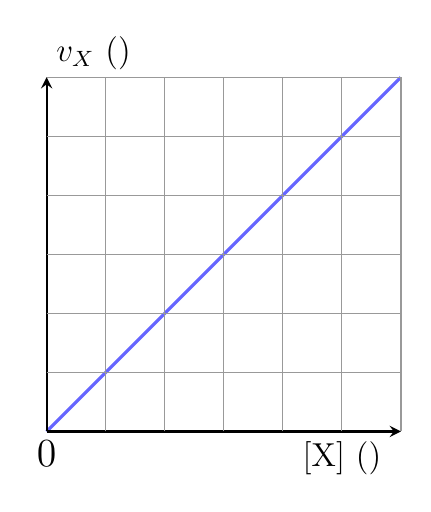
\begin{tikzpicture}[scale=1.5]%formation de produit
\draw [domain=0:3,samples = 300,blue!60,line width = 1.2pt] plot (\x,\x);
\draw (2.5,0) node[below]{\large[X] (\unit{\mole\per\liter})};
\draw (0,3.2) node[right]{\large $v_X$ (\unit{\mole\per\liter\per\second})};
\draw[-stealth,thick] (0,0) to (0,3);
\draw[-stealth,thick] (0,0) to (3,0);
\draw (0,0) node[below]{\Large 0};

\foreach \k in {.5,1,1.5,2,2.5,3} {
    \draw[gray!80] (\k,0) --(\k,3) ;
    \draw[gray!80] (0,\k) -- (3,\k);}
\end{tikzpicture}
    \end{minipage}
    
    \textbf{Conséquence sur la concentration :}\\
    Comme $v_{disp,R} = \dfrac{-d[R]}{dt}$, alors $\dfrac{-d[R]}{dt} = k\times [R]$ donc $\dfrac{d[R]}{dt} + k\times [R] = 0$.\\
    Cette équation différentielle admet comme solution : $[R](t)=[R]_0 \times e^{-kt}$ avec $[R]_0$ la concentration initiale en réactif $R$.\\
    \textbf{La concentration en réactif obéit donc à une loi exponentielle décroissante.}\\

    \textbf{Conséquence sur le temps de demi-réaction :}
    
    \begin{minipage}{.5\linewidth}
    Au bout de $t_{1/2}$, la concentration en réactif a diminué de moitié, donc : $[R](t_{1/2}) = \dfrac{[R]_0}{2}$. On aura donc : 
    $$[R]_0 \times \exp{-kt_{1/2}} = \dfrac{[R]_0}{2}$$
    $$\exp{-kt_{1/2}} =\frac{1}{2}$$
    $$\ln{\exp{-kt_{1/2}}} =\ln{\frac{1}{2}}$$
    $$-kt_{1/2} = \ln{1} -\ln{2}$$
    $$-kt_{1/2}=-\ln{2}$$
    $$ t_{1/2}=\dfrac{\ln{2}}{k}$$
    \end{minipage}
    \begin{minipage}{.4\linewidth}
        \centering
        \begin{tikzpicture}[scale=2]%formation de produit
            \draw [domain=0:3,samples = 300,blue!60,line width = 1.2pt] plot (\x,{3*exp(-3*\x)});
            \draw [domain=0:3,samples = 300,green!60!blue,line width = 1.2pt] plot (\x,{2*exp(-3*\x)});
            \draw[-stealth,thick] (0.0,0) to (0,3.2);
            \draw (3.2,0) node[below]{\large t (s)};
            \draw (0.231,0) node{$|$} node[below,red]{\Large $t_{1/2}$};
            \draw[dashed,red,line width = 1.2] (.231,1.5) to (0.231,0);
            \draw (0,3) node{$-$} node[left,blue!60]{\large $[A]_0$};
            \draw (0,1.5) node{$-$} node[left,blue!60]{\large $\dfrac{[A]_0}{2}$};
            \draw[dashed,red,line width = 1.2] (0,1.5) to (0.231,1.5);
            
            \draw (0,2) node{$-$} node[left,green!60!blue]{\large $[A]'_0$};
            \draw (0,1) node{$-$} node[below left,green!60!blue]{\large $\dfrac{[A]'_0}{2}$};
            \draw[dashed,red,line width = 1.2] (0,1) to (0.231,1);
            
            \draw (0,3.2) node[right]{\Large [A]};
            
            \foreach \k in {.5,1,1.5,2,2.5,3} {
                \draw[gray!80] (\k,0) --(\k,3) ;
                \draw[gray!80] (0,\k) -- (3,\k);}
            
            \draw[-stealth,thick] (0.0,0) to (3.2,0);
            \end{tikzpicture}
            
    \end{minipage}
    
    \textbf{Le temps de demi-réaction d'une transformation d'ordre 1 est indépendante de la concentration initiale de réactif.}\\
    L'ordre d'une réaction se déduire uniquement de l'expérience. \textbf{Les trois méthodes précédentes permettent de vérifier si une transformation est d'ordre 1.}

\newpage

\section{Mécanismes réactionnels}
	\subsection{Chocs efficaces}
Une réaction chimique ne peut avoir lieu que s'il y a contact entre deux entités chimiques. Lors de cette rencontre, la réaction chimique peut être décrite comme une réorganisation des atomes ou des charges électriques entre les deux entités. Cela implique des ruptures de liaisons covalentes ou des arrachages d'électrons avant la formation de nouvelles liaisons ou la récupération d'électrons.\\
Si on considère la réaction \ce{A2 + B2 -> 2AB}, elle nécessite la rupture d'une liaison \chemfig{A-A} et d'une liaison \chemfig{B-B} avant la formation de deux liaisons \chemfig{A-B}.\\
En modélisant la rencontre entre les espèces \ce{A2} et \ce{B2} par un \textbf{choc}, il faut que la somme des énergies de liaisons de deux molécules soit supérieure à la comme des énergies de liaison \chemfig{A-A} et \chemfig{B-B}.\\
Après le choc, les atomes séparés ses recombinent en formant deux molécules \ce{AB}. On dit alors que le choc est \textbf{efficace}.
\begin{figure}[h!]
    \centering
\subfloat[\textbf{Choc efficace}]{
    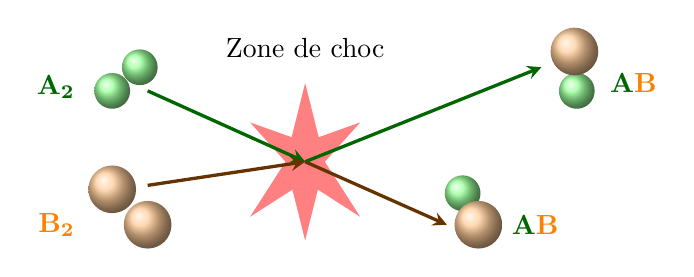
\begin{tikzpicture}[scale=1,transform shape]
    \fill[red!50] (2,1.8) -- (2.25,0.8) --  (2.7,.1) -- (2,.55) -- (1.3,.1) -- (1.75,.8) -- cycle;
    \fill[red!50] (2,-.2) -- (1.75,.8) --  (1.3,1.3) -- (2,1.05) -- (2.7,1.3) -- (2.25,.8) -- cycle;
    
    \shade[ball color=orange!40!white] (-0.45,.45) circle (2ex);
    \shade[ball color=orange!40!white] (0,0) circle (2ex);
    \shade[ball color=green!40!white] (-0.45,1.7) circle (1.5ex);
    \shade[ball color=green!40!white] (-.1,2) circle (1.5ex);
    
    \shade[ball color=green!40!white] (5.45,1.7) circle (1.5ex);
    \shade[ball color=orange!40!white] (5.42,2.2) circle (2ex);
    \shade[ball color=green!40!white] (4,.4) circle (1.5ex);
    \shade[ball color=orange!40!white] (4.2,0) circle (2ex);

    \draw[green!40!black,-stealth,very thick] (0,1.7) to (2,.8);
    \draw[green!40!black,-stealth,very thick] (2,.8) to (5,2);
    \draw[orange!40!black,-stealth,very thick] (0,.5) to (2,.8);
    \draw[orange!40!black,-stealth,very thick] (2,.8) to (3.8,0);

    \draw (2,2) node[above]{Zone de choc};
    \draw (-.8,0) node[left]{\textcolor{orange}{$\mathbf{B_2}$}};
    \draw (-.8,1.75) node[left]{\textcolor{green!40!black}{$\mathbf{A_2}$}};
    \draw (5.75,1.8) node[right]{\textcolor{green!40!black}{$\mathbf{A}$}\textcolor{orange}{$\mathbf{B}$}};
    \draw (4.5,0) node[right]{\textcolor{green!40!black}{$\mathbf{A}$}\textcolor{orange}{$\mathbf{B}$}};
\end{tikzpicture}
}
\subfloat[\textbf{Choc inefficace}]{
    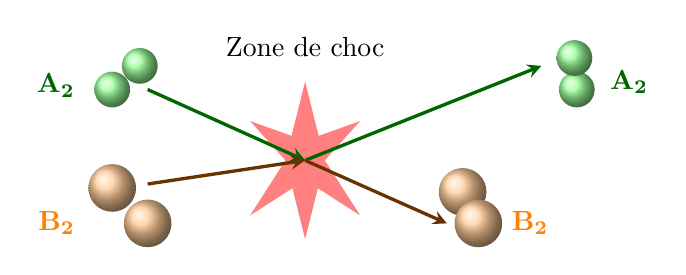
\begin{tikzpicture}[scale=1,transform shape]
    \fill[red!50] (2,1.8) -- (2.25,0.8) --  (2.7,.1) -- (2,.55) -- (1.3,.1) -- (1.75,.8) -- cycle;
    \fill[red!50] (2,-.2) -- (1.75,.8) --  (1.3,1.3) -- (2,1.05) -- (2.7,1.3) -- (2.25,.8) -- cycle;
    
    \shade[ball color=orange!40!white] (-0.45,.45) circle (2ex);
    \shade[ball color=orange!40!white] (0,0) circle (2ex);
    \shade[ball color=green!40!white] (-0.45,1.7) circle (1.5ex);
    \shade[ball color=green!40!white] (-.1,2) circle (1.5ex);

    
    \shade[ball color=green!40!white] (5.45,1.7) circle (1.5ex);
    \shade[ball color=green!40!white] (5.42,2.1) circle (1.5ex);
    \shade[ball color=orange!40!white] (4,.4) circle (2ex);
    \shade[ball color=orange!40!white] (4.2,0) circle (2ex);

    \draw[green!40!black,-stealth,very thick] (0,1.7) to (2,.8);
    \draw[green!40!black,-stealth,very thick] (2,.8) to (5,2);
    \draw[orange!40!black,-stealth,very thick] (0,.5) to (2,.8);
    \draw[orange!40!black,-stealth,very thick] (2,.8) to (3.8,0);

    \draw (2,2) node[above]{Zone de choc};
    \draw (-.8,0) node[left]{\textcolor{orange}{$\mathbf{B_2}$}};
    \draw (-.8,1.75) node[left]{\textcolor{green!40!black}{$\mathbf{A_2}$}};
    \draw (5.75,1.8) node[right]{\textcolor{green!40!black}{$\mathbf{A_2}$}};
    \draw (4.5,0) node[right]{\textcolor{orange}{$\mathbf{B_2}$}};
\end{tikzpicture}
}
%\caption*{(a) \textbf{Choc efficace} (b) \textbf{Choc inefficace}}
\end{figure}

Un \textbf{acte élémentaire} est une réaction se déroulant à l'échelle microscopique en une seule étape, modélisée par un \textbf{choc efficace} entre deux entités chimiques.

	\subsection{Mécanismes réactionnels}
A l'échelle microscopique, le passage des réactifs aux produits se décompose en une succession d'actes élémentaires. Pour une réaction chimique \textbf{complexe}, on appelle cette succession d'actes élémentaires le \textbf{mécanisme réactionnel}.
		\subsubsection{Intermédiaires réactionnels et catalyseur}
Lorsque l'on étudie le mécanisme réactionnel, celui-ci peut faire apparaître un intermédiaire réactionnel : une entité chimique initialement absente de la réaction, qui n'est pas dans l'équation de réaction et qui a une durée de vie très courte, il est produit dans un acte élémentaire et disparaît dans un acte suivant. ou un catalyseur : une entité chimique initialement présente dans le système, qui ne figure pas dans l'équation de réaction, qui réagit dans un acte élémentaire et est régénéré dans un acte suivant.\\

\begin{table}[h!]
    \centering
    \caption*{\textbf{Exemple 1 : Réaction du diazote avec le monoxyde de carbone}}
    \begin{tabular}{>{\centering}m{.2\linewidth} >{\centering\arraybackslash}m{.5\linewidth}}
        Acte élémentaire 1 :& \ce{NO2 + NO2 -> \textbf{\ce{NO3}} + NO}\\
        Acte élémentaire 2 :& \ce{CO + NO3 -> CO2 + NO2}\\ \hline
        Bilan :& \ce{NO2 + CO -> NO + CO2}\\
    \end{tabular}
    \label{tab:ex1}
\end{table}
\textbf{\ce{NO3}} est un intermédiaire réactionnel car il est absent dans le mélange initial, il est créé à l'acte 1 et il disparaît dans l'acte 2.
\begin{table}[h!]
    \centering
    \caption*{\textbf{Exemple 2 : Réaction d'estérification}}
    \begin{tabular}{>{\centering}m{.2\linewidth} >{\centering\arraybackslash}m{.5\linewidth}}
Acte élémentaire 1 :& \ce{C4H8O2 + H+ -> C4H9O2+}\\
Acte élémentaire 2 :& \ce{C4H9O2+ + CH4O -> C5H13O3+}\\
Acte élémentaire 3 :& \ce{C5H13O3+ -> C5H10O2+H2O + H+}\\
\hline
Bilan :& \ce{C4H8O2 + CH4O -> C5H20O2 + H2O}\\
\end{tabular}
    \label{tab:ex2}
\end{table}
\ce{C4H9O2+} et \ce{C5H13O3+} sont des intermédiaires réactionnels, ils sont absents dans le mélange initial, apparaissent dans un acte élémentaire et disparaissent dans le suivant.\\
\ce{H+} est un catalyseur, il est présent dans le mélange initial, disparaît dans l'acte 1 et est régénéré dans l'acte 3.\\
Les produits de l'estérification de l'acide butanoïque \ce{C4H8O2} avec le méthanol \ce{CH4O} sont le butanoate de méthyle \ce{C5H10O2} et l'eau \ce{H2O}.

\subsection{Sites donneurs, accepteurs et flèches courbes}
        \subsubsection{Présence des sites donneurs et accepteurs}
Lorsque deux entités se rapprochent, les forces prédominantes, à cette échelle sont les forces d'interaction électrostatiques. Pour prévoir la manière dont les entités vont interagir, il faut pouvoir identifier la répartition de leurs charges électriques.\\
L'\textbf{électronégativité $\mathbf{\chi}$} d'un élément chimique est une mesure de sa capacité à attirer à lui les électrons d'une liaison de valence. Si la différence d'électronégativité entre deux atomes liés est supérieure ou égale à 0,4, la liaison est \textbf{polarisée}. L'atome le plus électronégatif porte alors une \textbf{charge électrique partielle} négative $\delta^-$, l'atome le moins électronégatif porte une charge électrique partielle $\delta^+$.\\

\begin{figure}[h!]
\centering
\subfloat[\textbf{Charges partielles}]{
	\begin{minipage}{.25\linewidth}
	\centering
    \chemfig{\charge{200[anchor=180+\chargeangle]=$\delta^+$}{H}-\charge{-20[anchor=180+\chargeangle]=$\delta^-$}{Cl}}
    \end{minipage}
}
\subfloat[\textbf{Attaque d'un doublet non liant}]{
	\begin{minipage}{.5\linewidth}
	\centering
    \schemestart
 	\chemfig[atom sep=2em]{H-C(-[:90]H)(-[:-90]H)-@{dnl}\charge{-120[anchor=180+\chargeangle]=$\delta^-$,35=\|,125=\|}{O}-[:-35]\charge{-60[anchor=180+\chargeangle]=$\delta^+$}{H}} 
 	\chemfig{@{atoh}\charge{60[anchor=180+\chargeangle]=$+$}{H}}
 	\arrow{->}
 	\chemfig[atom sep=2em]{H-C(-[2]H)(-[6]H)-\charge{45[anchor=180+\chargeangle]=$+$,90[anchor=180+\chargeangle]=\|}{O}(-[6]H)-H}
 	\schemestop
  	\chemmove{
 		\draw[shorten <=2pt, shorten >=7pt]
 	(dnl).. controls +(north east:1cm) and +(north west:1cm).. (atoh);}
 	\end{minipage}
 }
%\caption*{(a) Charges partielles (b) Attaque d'un doublet non liant}
\end{figure}
Un \textbf{site} est un lieu précis dans une entité chimique, atome, doublet d'électrons liant ou non liant. Un \textbf{site donneur} d'électrons est un site riche ou excédentaire en électrons : doublet non liant d'électrons, liaison double ou triple, atome portant une charge électrique ionique ou partielle négative. Un \textbf{site accepteur} d'électrons est un site pauvre ou en déficit d'électrons : un atome portant une charge ionique ou partielle positive.
        \subsubsection{Flèches courbes}
Lorsque deux espèces réactives se rencontrent, une force électrostatique attractive s'exerce entre les sites donneurs et les sites accepteurs.\\
Un acte élémentaire peut être expliqué par l'\textbf{attaque} d'un site donneur sur un site accepteur d'électrons. On schématise cette attaque par une \textbf{flèche courbe} tracée très précisément entre le site donneur (début de la flèche) et le site accepteur (pointe de la flèche).

\subsection{Interprétation de l'influence des facteurs cinétiques}
    \subsubsection{La concentration}
L'augmentation de la concentration des réactifs se traduit par des collisions plus fréquentes entre les espèces réactives, et donc par une augmentation de la vitesse de disparition des réactifs.
    \subsubsection{La température}
L'augmentation de la température se traduit par une agitation plus importante des entités. Elle a donc un double effet :
\begin{itemize*}
    \item les \textbf{collisions} entre les espèces réactives dont  \textbf{plus fréquentes}
    \item les \textbf{chocs} sont plus violents donc plus souvent efficaces.
\end{itemize*}
La vitesse d'apparition des réactifs est donc plus grande.
    \subsubsection{Catalyseur}
L'ajout d'un catalyseur modifie le mécanisme réactionnel d'une réaction, en remplaçant une duite d'actes lents en une suite d'actes plus \textbf{rapides}.







\end{document}